\section{GameController Arkitektur}
Game Controllerns rolle er at skabe logikken for brugeren i spillet. Game Controllerens rolle for systemet er afgørende, når spillet er startet for brugeren. Game Controllerens funktionalitet indebærer blandt andet at skabe et map for brugeren, så spilleren kan flytte fra rum til rum ved start af spil. Her forekommer det at brugeren anvender Front End til at interagere med spillet og derefter kan funktionerne fra Game Controlleren kaldes.
\subsection{States og Character interagering}
\begin{figure}[H]
\centering
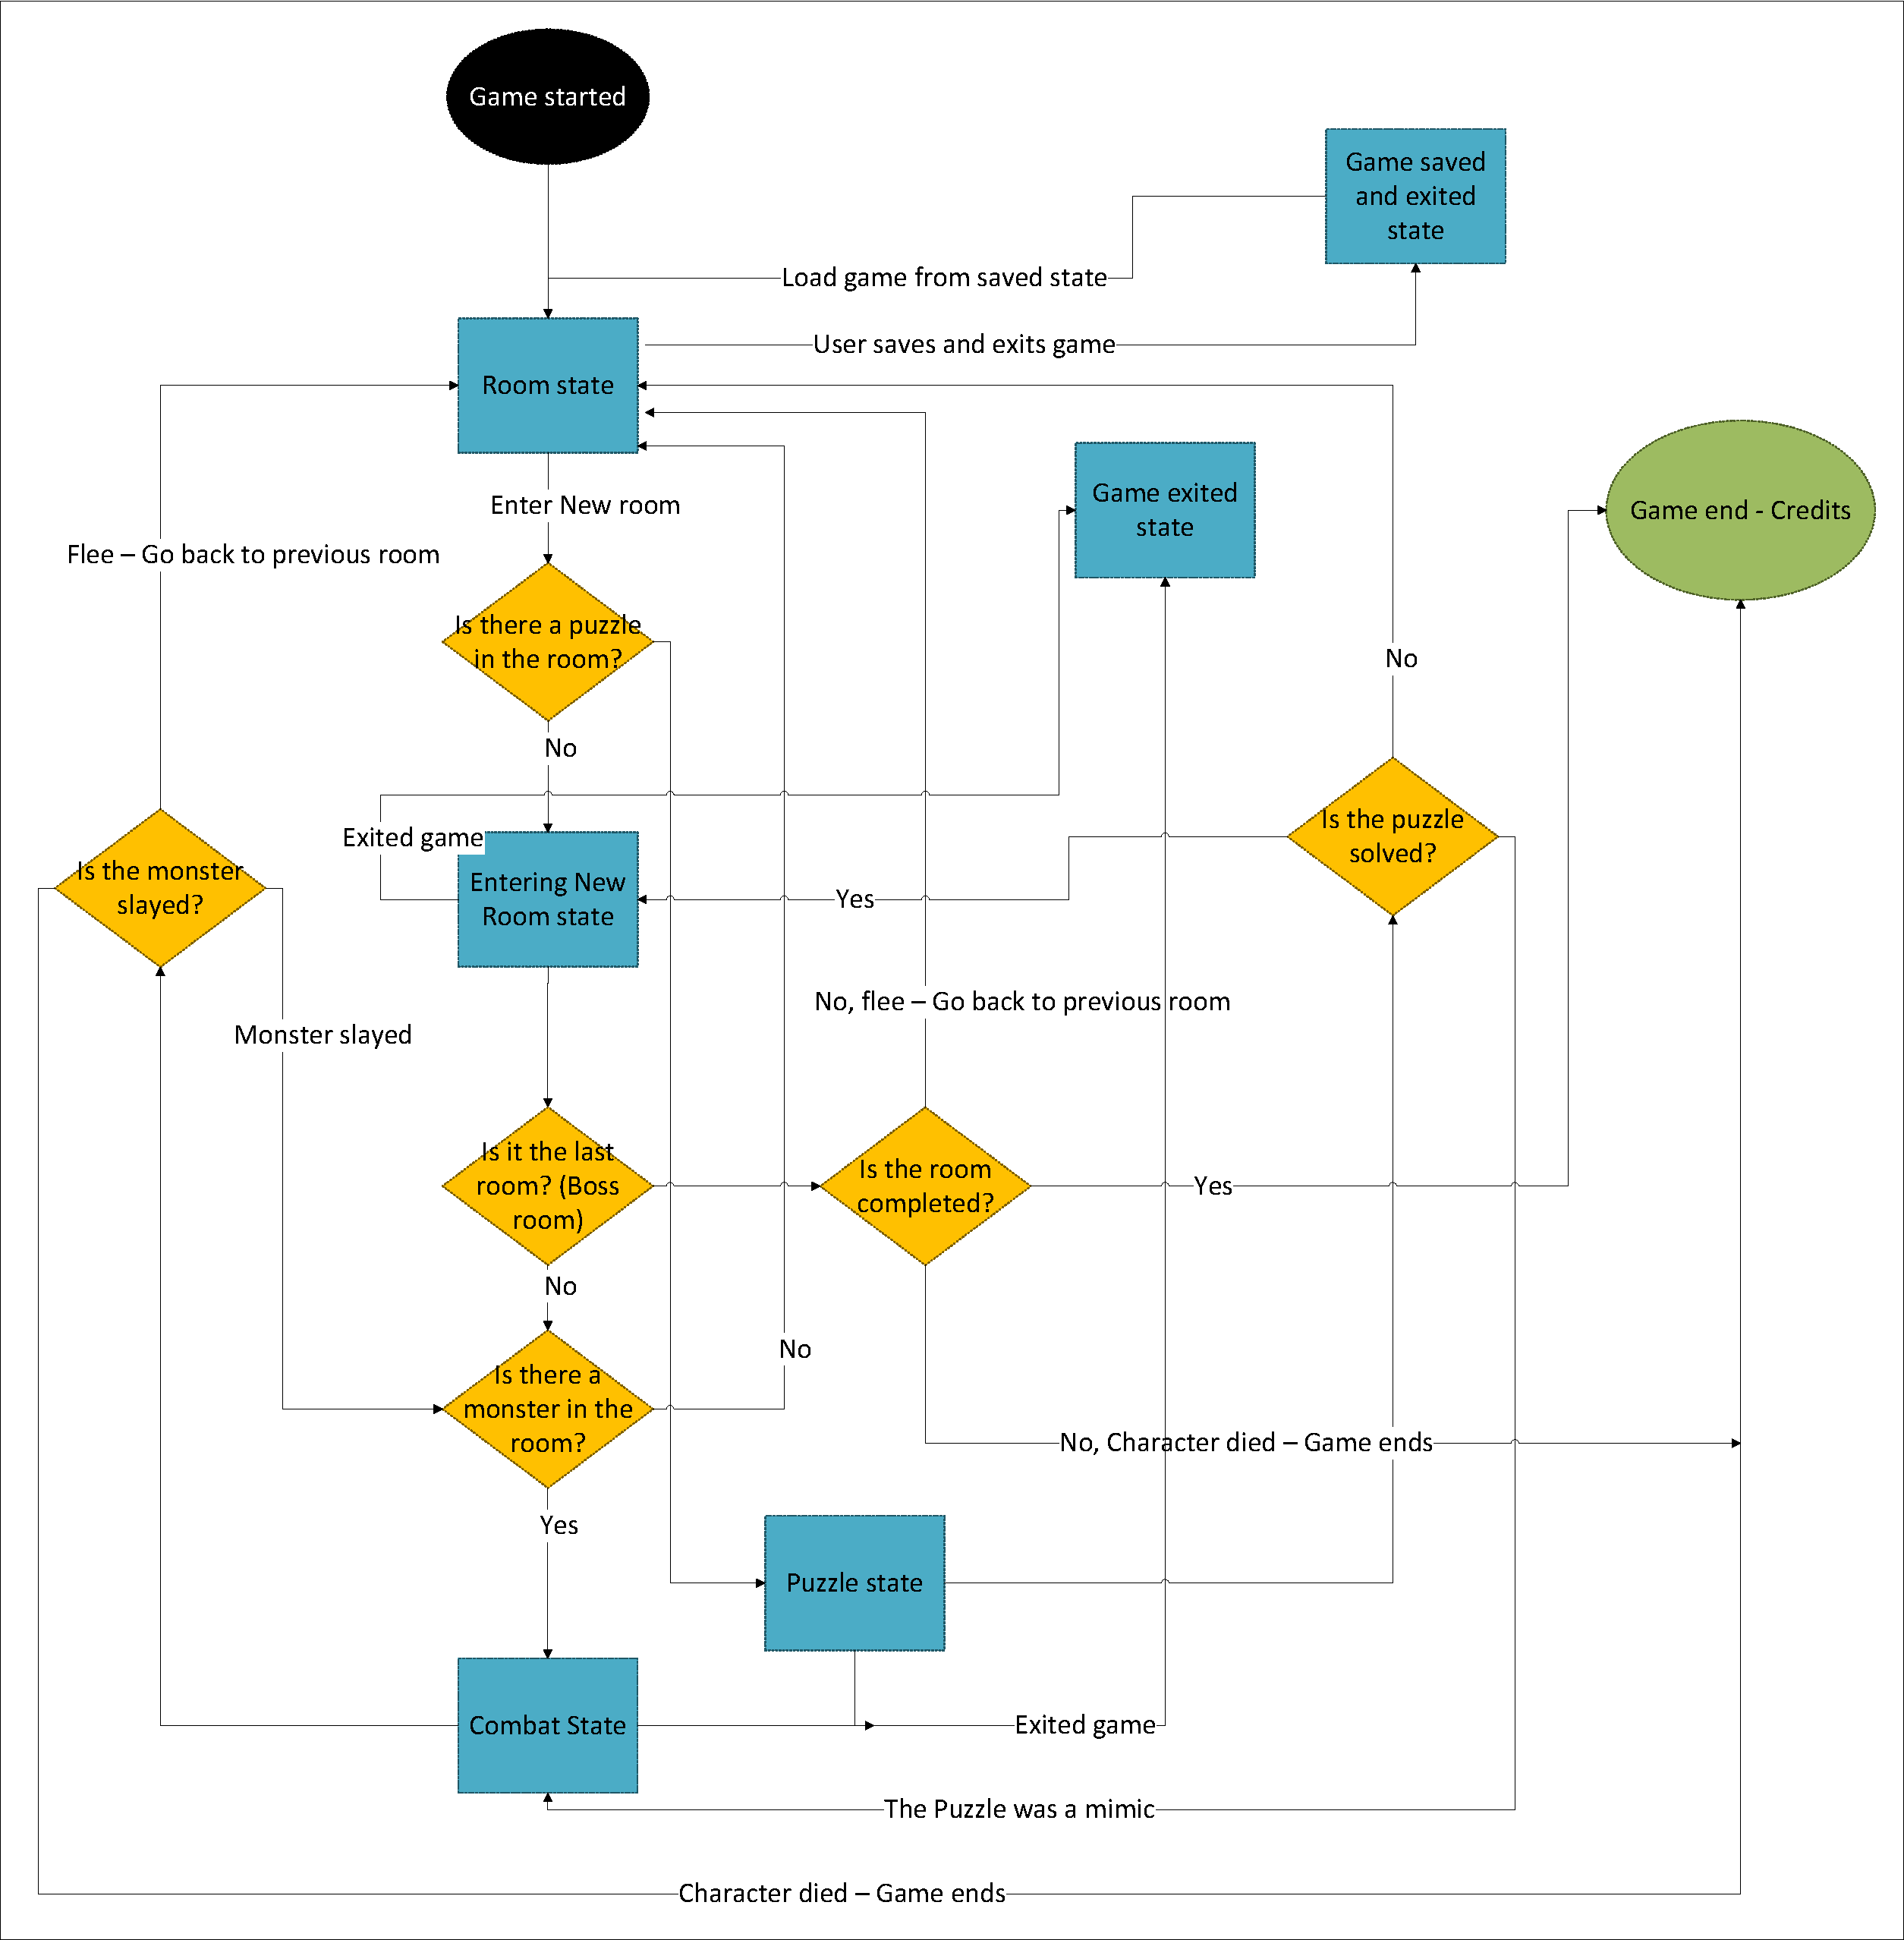
\includegraphics[width = \textwidth]{02-Body/Images/Arkitektur - State Logic.pdf}
\caption{Flow Chart over systemets states når spillet er startet. Dette bilag viser arkitekturen over det ønskede states i systemet når bruger har startet spillet. Dette viser også hvordan spillets fremgang er ønsket og hvordan bruger kommer videre i spillet igennem de forskellige states.}
\label{fig:Arkitektur-SD-SaveGame}
\end{figure}
\subsection{Room State og Character interagering}
Det andet som Game controlleren har ansvaret for, er spillerens våben og skjold. Game Controlleren er delt op i spillets game states som kan ses i bilaget ovenover. Der er hovedsageligt 2 states når spillet er startet. Room State og Combat state. Når spillet er startet for brugeren, starter brugeren i et room state. I dette state kan der interageres med rummet, hvis der er genstande til stede. Her kan brugeren også brugerdefinere sin spiller ved brug af knappen inventory og skifte våben eller skjold. Her kan der også se spillerens evner ved brug af knappen Character. Derudover er der også implementeret beskrivelser fra de forskellige rum som hentes fra modulet Database via modulet Back end.
\subsection{Combat State og Combat simulering}
Combat state indebærer når spilleren møder en fjende. Dette sker når man går ind i forskellige rum. Der er oprettet klasser for spillerens evner i form af Attack(Spillerens evne til at slå) og Armor(Spillerens evne til at modstå angreb). Når spilleren angriber en fjende foregår det ved at brugeren trykker på knappen ’Attack’. Når dette forekommer er der implementeret en terning i Game Controlleren. Dette skal implementeres ved to implementeringer. En simuleret terning i form af en pseudo random-number generator som genererer et tal mellem 1 og parameteren numOfSides og en  En Rekursive Psudo-Random number generator som tager en tuple (numOfSides, numOfDice). Den gentager rekursivt implementering 1. Et antal gange svarende til NumOfDice parameteren og summere alle resultaterne.  Hvis brugeren taber kampen, skal brugeren starte et nyt spil eller loade et save. I figuren under ses et Flow chart over forløbet når spiller går ind i combat state.
\begin{figure}[H]
\centering
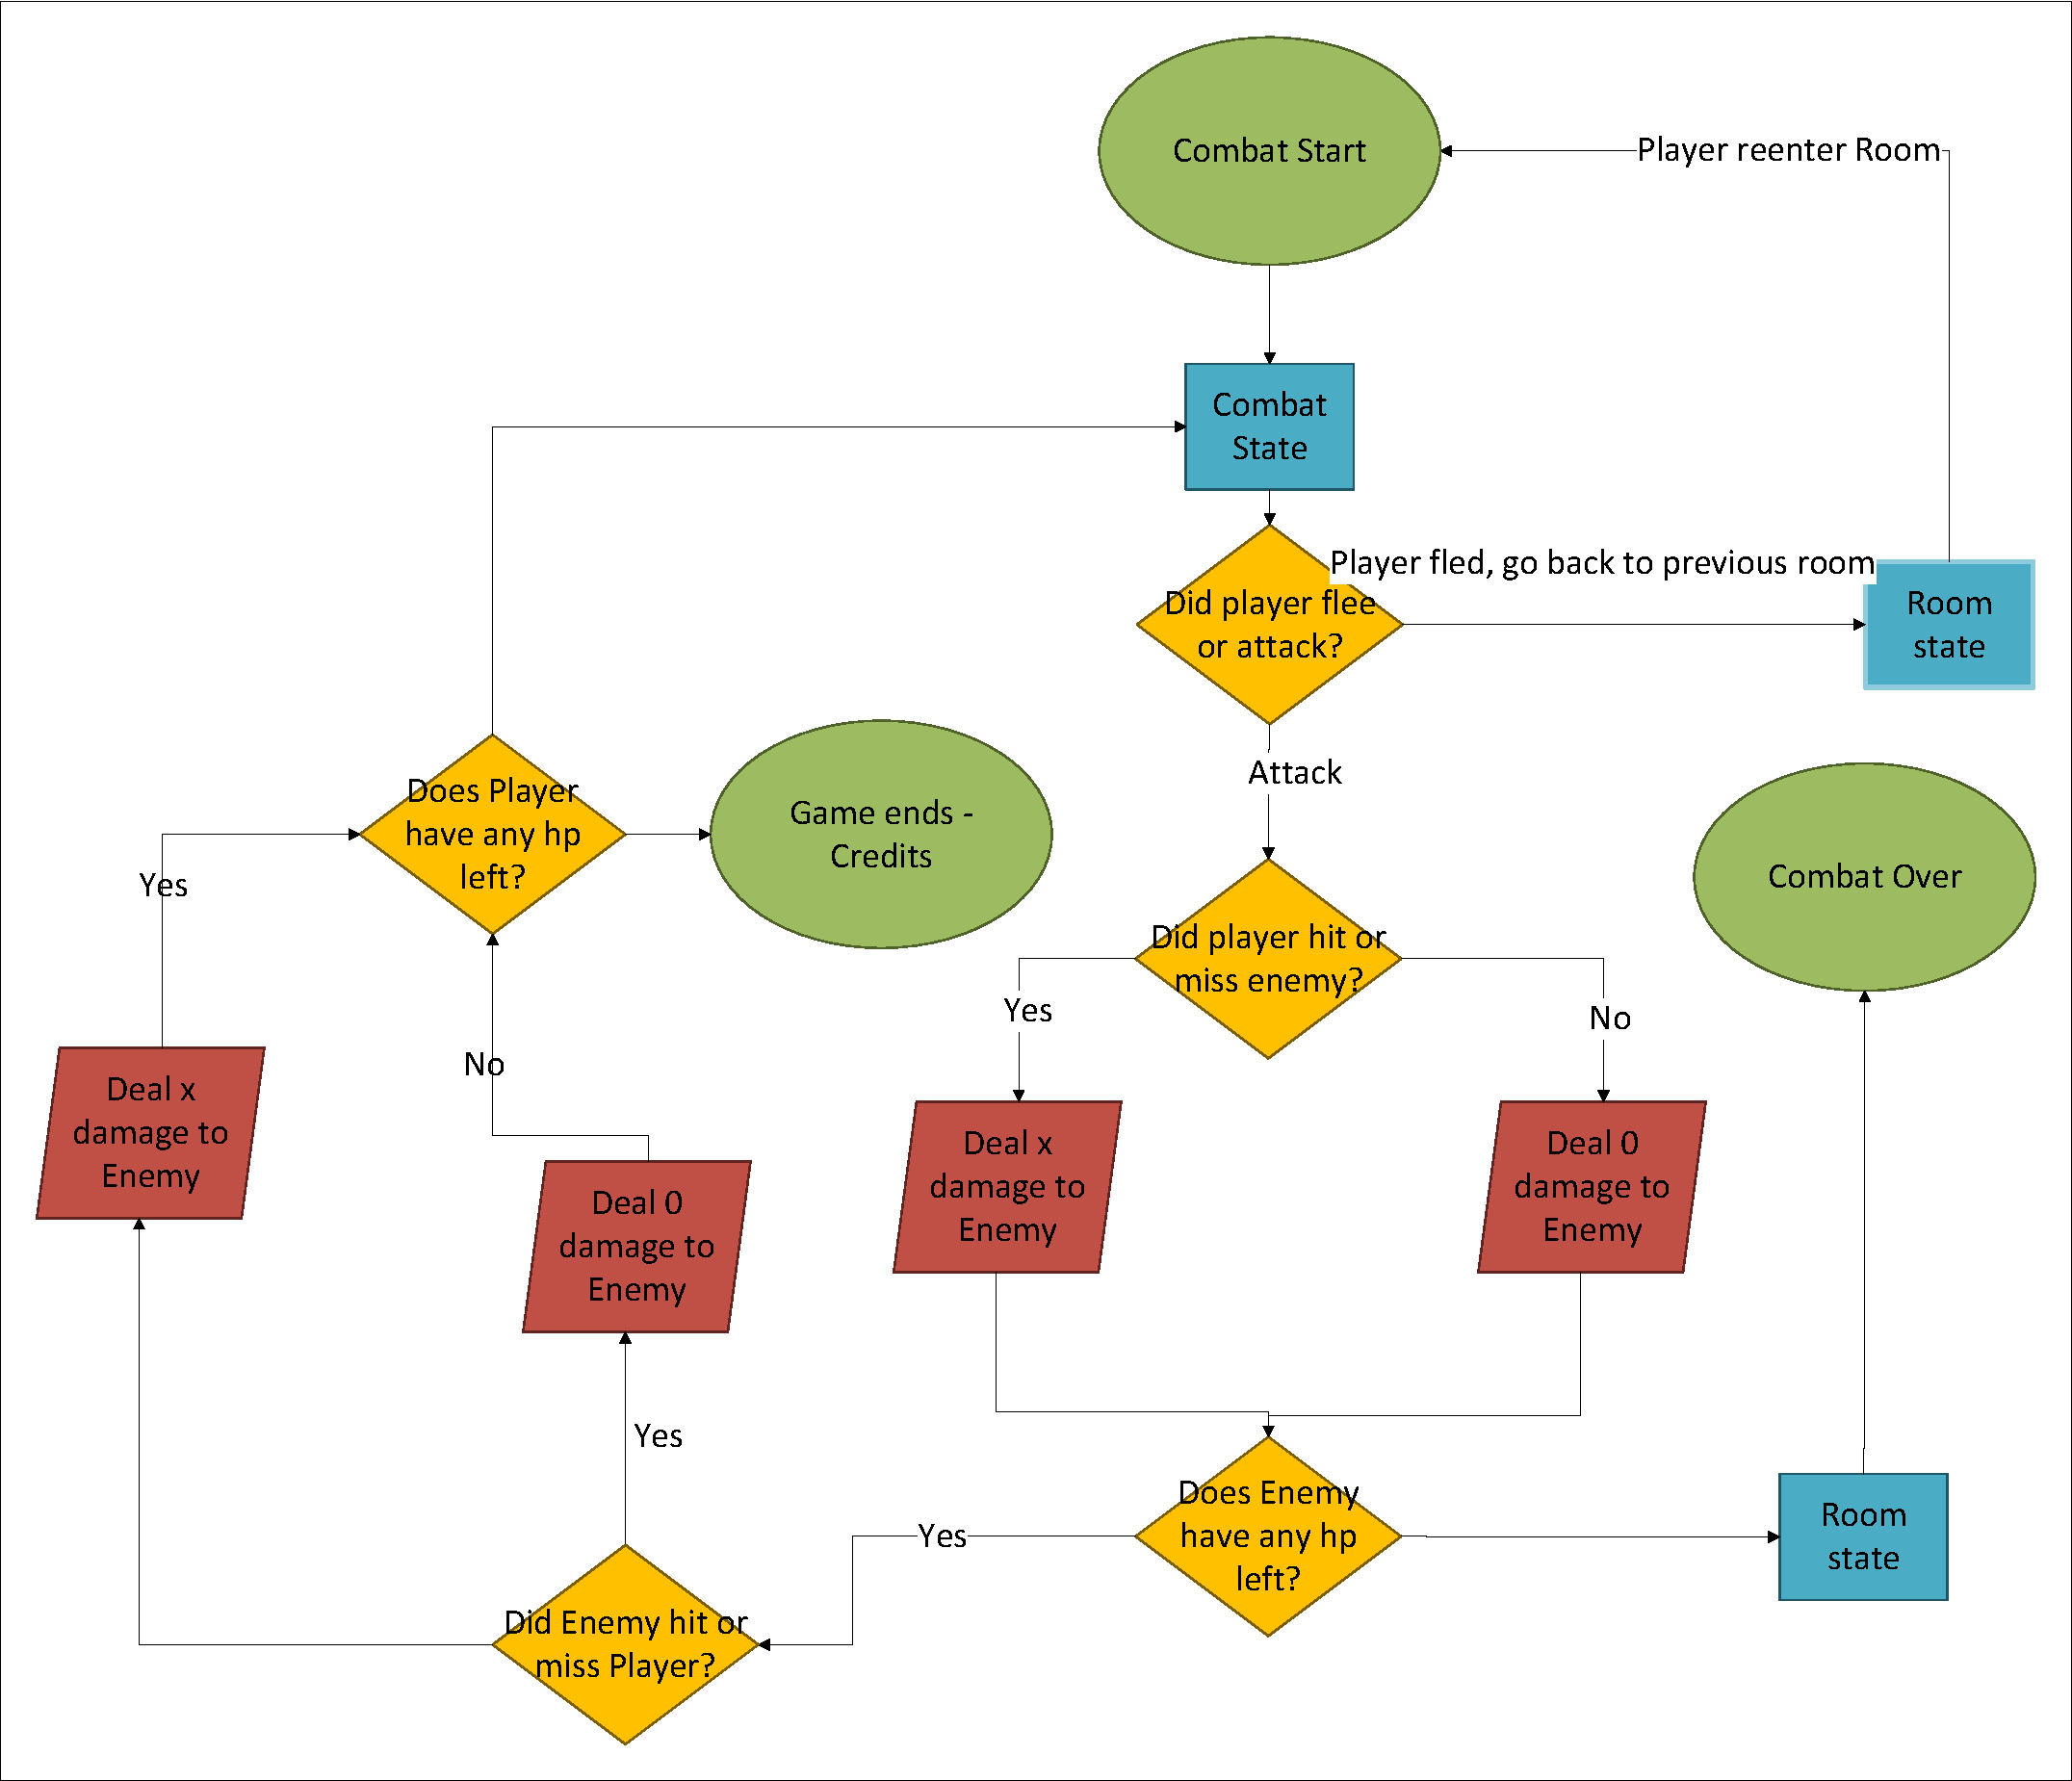
\includegraphics[width = \textwidth]{02-Body/Images/Arkitektur - Combat State.pdf}
\caption{Flow Chart over spillets fremgang når spiller går ind i combat State. Når spiller går ind i et rum med en fjende i rummet, går spillet ind i combat state. Herfra skal spillets terning simulerer et tilfældigt nummer ud fra spilllerens evner. Fjendens evner er bestemt i forvejen. Angreb fastlægges om spiller ruller højere end fjendens Armor Class og vice versa De tre outcomes for spilleren er følgende: Spiller flygter(flee-knap), Spilleren mister alt liv(Spil sluttes) og fjende mister alt liv(Spiller går til room state)}
\label{fig:Arkitektur-SD-SaveGame}
\end{figure}
\subsection{Forbindelser til andre moduler}
Game Controlleren er forbundet med systemets Back-end og Front-End. Den håndterer data fra Back-end som derefter kan håndteres, så Front-end kan kalde funktionerne fra Game Controlleren. Det data som skal håndteres er primært gemmets forløb som kan lagres i databasen under brugeren. Herefter kan bruger loade det samme gem igen med samme fremgang som da bruger gemte spillet. Det vil være nuværende rum, rum der er blevet besøgt, fjender der er blevet bekæmpet og genstande der er samlet op og taget på.